\documentclass[11pt,nswissgerman]{article}
\usepackage{helvet}
\renewcommand{\familydefault}{\sfdefault}
\usepackage[latin2]{inputenc}
\usepackage[a4paper]{geometry}
\geometry{verbose,tmargin=3cm,bmargin=3cm,lmargin=3.5cm,rmargin=3.5cm,headheight=3cm,headsep=1cm,footskip=2cm}
\usepackage{fancyhdr}
\pagestyle{fancy}
\usepackage{wrapfig}
\usepackage{graphicx}
\usepackage[position=bottom]{subfig}
\usepackage{titletoc}
\usepackage{float}
\makeatletter
\@ifundefined{date}{}{\date{}}
\makeatother
\usepackage{babel}
\usepackage[
            colorlinks=true,
            urlcolor=green,
            linkcolor=black
]{hyperref}
\setcounter{secnumdepth}{1} % levels under \section are not numbered
\setcounter{tocdepth}{2}    % levels under \subsection are not listed in the TOC
\begin{document}
\author{Stefan Bopp}
\title{\Huge Tagebuch Gruyere 2016\vspace{2cm}

\includegraphics[width=0.4\textwidth]{../Bilder/Logo/Logo.png}
}
\maketitle
\vfill
\tableofcontents

\newpage

\lhead{Gruyere 2016}

\rhead{jackthebus.com}

\cfoot{\thepage}
%    JJJ    AA     CCCCCC KKK   K TTTTTT HH  HH EEEEEE BBBBBB UU  UU SSSSSS    CCCCCC OOOOOO MM  MM
%    JJJ   AAAA    CCCCCC KKK  K  TTTTTT HH  HH EEEEEE BB   B UU  UU SSS       CCCCCC OOOOOO MM  MM
%    JJJ  AA  AA   CC     KKK K     TT   HHHHHH EEE    BB   B UU  UU SSS       CC     OO  OO MMMMMM
%    JJJ AA    AA  CC     KKKK      TT   HHHHHH EEEEEE BBBBBB UU  UU  SSSSS    CC     OO  OO M MM M
%    JJJ AAAAAAAA  CC     KKK K     TT   HH  HH EEE    BB   B UU  UU    SSS    CC     OO  OO M MM M
% JJJJJJ AA    AA  CCCCCC KKK  K    TT   HH  HH EEEEEE BB   B UUUUUU    SSS .. CCCCCC OOOOOO M MM M
% JJJJJJ AA    AA  CCCCCC KKK   K   TT   HH  HH EEEEEE BBBBBB UUUUUU SSSSSS .. CCCCCC OOOOOO M MM M
% 
% Texte Geschrieben von Stefan Bopp und Chantal Frunz
% Mehr Informationen sind auf jackthebus.com zu finden

\subsection{05.05.2016 Ankunft im Welschland}

\begin{wrapfigure}{R}{0.45\textwidth} 
  \begin{centering}
    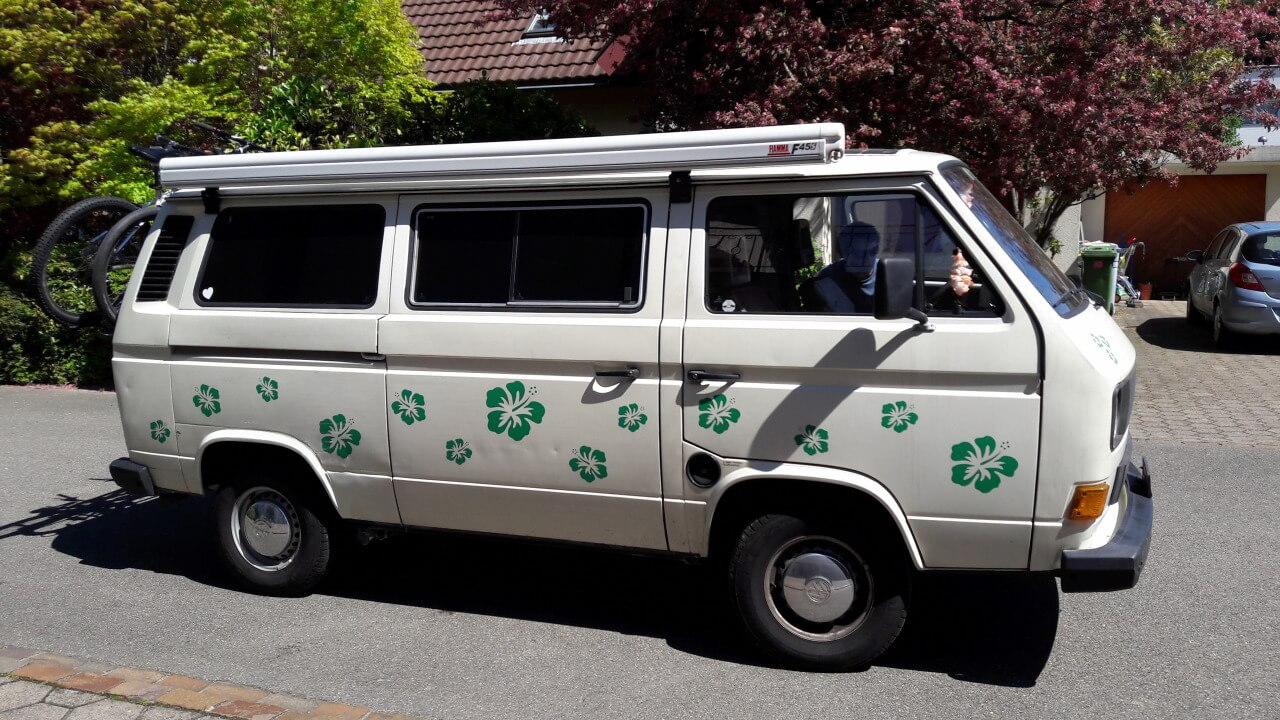
\includegraphics[width=0.4\textwidth, height=5cm, keepaspectratio]{../Bilder/Gruyere/1.jpg}
    \caption{Abfahrt}
  \end{centering}
\end{wrapfigure} 


Zuerst musste Gep�ck Fahrr�der Personen und der Bus zusammen gebracht werden.
Alles von Luzern nach Nussbaumen, wo der Bus auf uns wartete.
Einmal alles umladen und los ging die Fahrt in das f�r uns unbekannte Welschland.
So unbekannt war die Region f�r mich jedoch nicht.
Durfte ich doch 21 Wochen bezahlt von Vater Staat in der Region Payerne verbringen.
Diese Aufenthalte f�rdern den Ruf einer Gegend normalerweise nicht sonderlich.
Zus�tzlich wird gemunkelt, dass in der Region eine sehr komplizierte Sprache gesprochen wird.
Dieser Sprache m�chtig zu werden bedarf einiges an Magie, einer gesunden Portion Verr�cktheit und sonst eines am L�ffel.

Nach kurzem Stau auf der Autobahn zeigten sich die Berner Alpen am Horizont bei wunderbarer Fernsicht.
Der Campingplatz w�rde Dank modernster Navigationsmittel problemlos gefunden und die Reihe vor der Rezeption glich einer Bus-Parade.
Der Versprochene Platz direkt am See war dann auch Wirklichkeit (Dank Reservation) und ein kleines Restaurant direkt am Campingplatz sollte uns mit Speisen und Trank versorgen k�nnen.

\begin{wrapfigure}{L}{0.45\textwidth} 
  \begin{centering}
    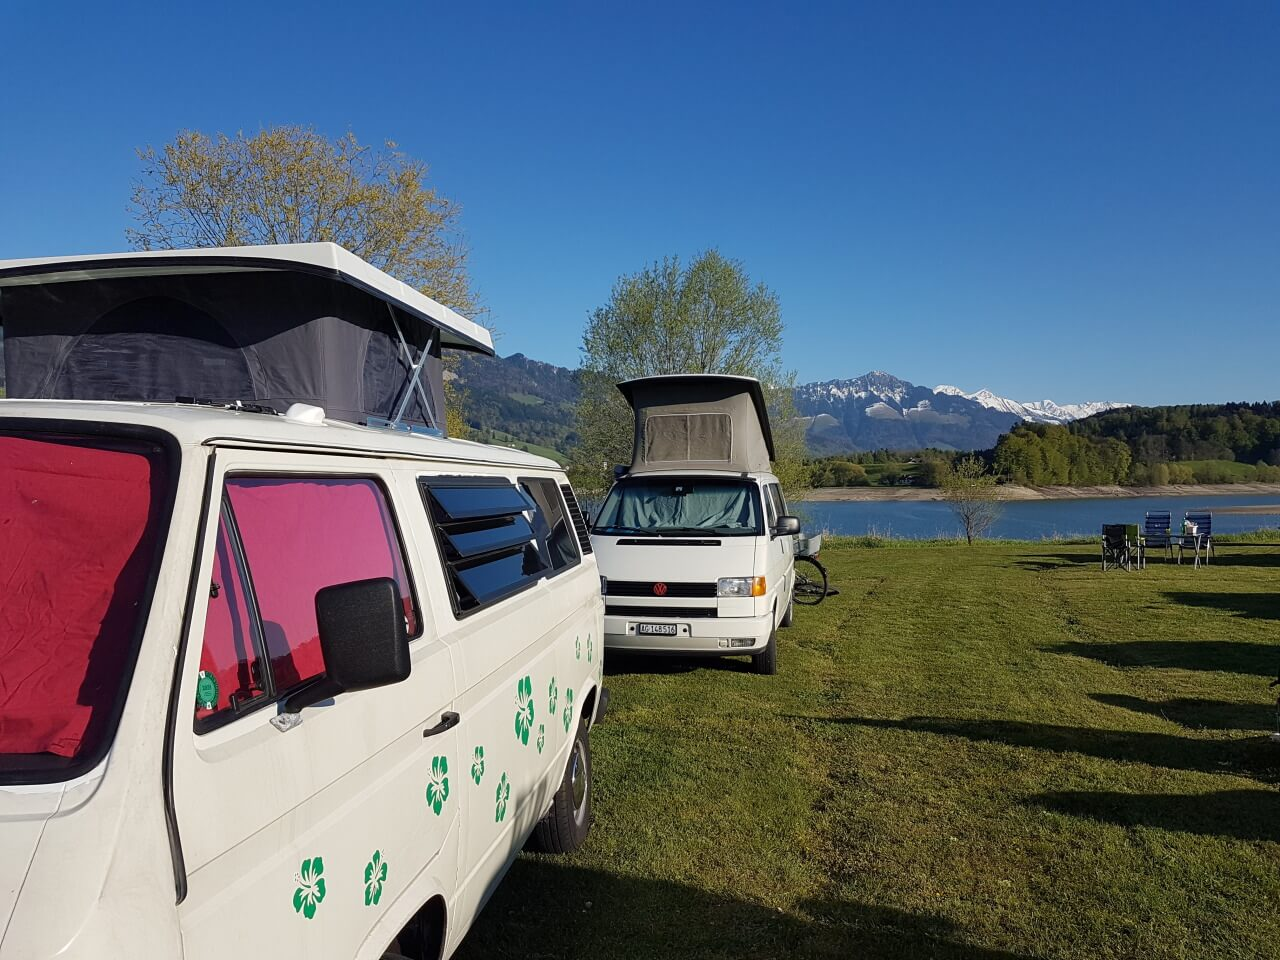
\includegraphics[width=0.4\textwidth, height=5cm, keepaspectratio]{../Bilder/Gruyere/5.jpg}
    \caption{Einreihen}
  \end{centering}
\end{wrapfigure} 

Nach dem Aufstellen und einem kurzen Spaziergang am See, welcher ich zur Zeit vor allem mit einem sehr tiefen Wasserstand bemerkbar macht, kam die Einsicht, dass das ganze mit dem Strom f�r unseren Ofen eine eher schwierige Angelegenheit wird.
Die Standpl�tze selbst waren nicht mit einer eigenen Stromversorgung ausger�stet, sondern es stand ein Bau-Provisorium in einer Ecke.
Der Rest der Verteilung des Stromes war dann dem Zufall �berlassen.
Gerade die kalte Nacht, welche auf uns wartete, erh�hte die Wahrscheinlichkeit des Scheiterns des Systems erheblich.
Sowieso waren leider die Pl�tze am See noch gar nicht erschlossen.
So wurde entschieden die Nacht ohne Ofen zu verbringen.
Sind ja nicht aus Zucker.
Das Restaurant trumpfe gross auf.
Mit einem 300 gr. Steak auf dem hei�en Stein und Wein im �berfluss machte es bei mir sehr viele Punkte gut.
Nach einem Test des neuen Multimediasystem des Buses hie� es sich warm einzupacken und seit langer Zeit wieder einmal im Bus zu schlafen.

\begin{figure}[hb]
    \centering
    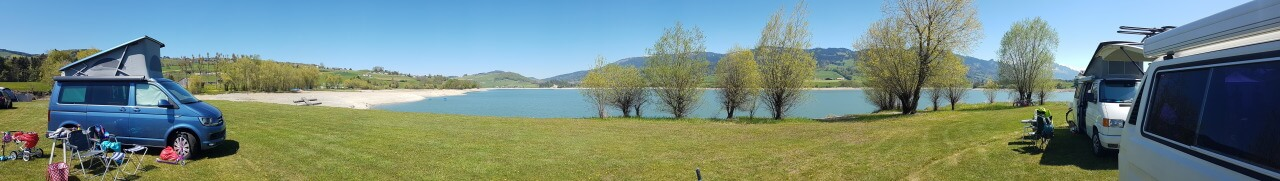
\includegraphics[width=\textwidth]{../Bilder/Gruyere/3.jpg}
    \caption{Platz am See}
    \label{img:Flims}
\end{figure}

\subsection{06.05.2016 St�rmt das Schloss Gruy\`{e}res}

\begin{wrapfigure}{L}{0.45\textwidth} 
  \begin{centering}
    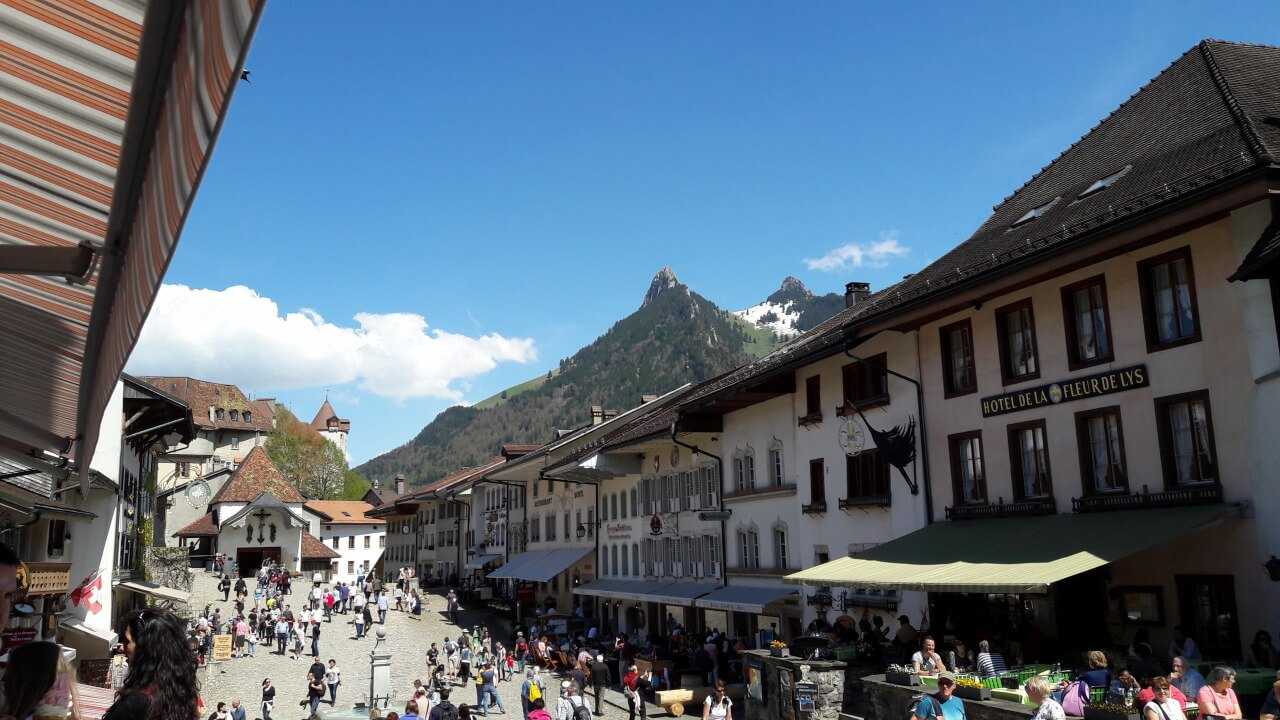
\includegraphics[width=0.4\textwidth, height=5cm, keepaspectratio]{../Bilder/Gruyere/10.jpg}
    \caption{Gruyere}
  \end{centering}
\end{wrapfigure} 

Oh ja, Herstellerangaben sollte man glauben.
Der Comfort-Bereich meines Schlafsack ist bei warmen 13�C nach unten beschr�nkt.
Die klare Nacht hielt nichts von diesem Limit und n�herte sich erbarmungslos der 0� Grenze.
Gegen Null ging auch die Laune von Chantal nach dem ich sie unter einer Unmenge von Decke am Morgen nach ihrem Befinden fragte.
Ne, eine weiter Nacht ohne w�rmenden Ofen kommt nicht in Frage.
So konnte die Frage nach Strom ganz zu oberst auf der Priorit�tenliste gefunden werden.
Nach mehrmaligen hin und her fanden wir dann auch einen freien Steckplatz in dem nach asiatischen Vorbild nat�rlich gewachsenen Stromnetz.
Die Warnung, dass an diesem Knoten bereits 3 Ofen angeschlossen seien, stimmte nicht gerade zuversichtlich.
Man wird sehen.
Nach einem reichhaltigen Fr�hst�ck direkt am See wurden Pl�ne f�r eine Velotour geschmiedet.
Rucks�cke gepackt Google Maps nach der Route befragt und los kann es gehen.

Die anf�ngliche Route der Hauptstra�e entlang k�nnte nicht begeistern und so wurde schon bald ein Abzweiger gefunden, welcher uns die typische Gegend n�her bringen sollte.
Nicht gerade Zielgerichtet ging es voran, aber immerhin sch�n ruhig und sehenswert.
Pools scheine hier niemanden zu Interessieren.
Daf�r Trampolins.
Jeder der was auf sich h�lt hat so ein Unget�m im Garten.
Beim ersten Abchecken der Karte wurde ein Bewohner sofort auf uns aufmerksam und fragte nach ob alles in Ordnung sei.
�berall sehr nette Menschen.
So ging es weiter mit einer Zusatzschlaufe zum Chocolatier Cailler.
Schon bald war die Sicht frei auf das Schloss Gruy\`{e}res.
Nur noch ein Flugplatz war im Weg.
Der wurde prompt f�r eine Zwischenverpflegung genutzt.
Ein Fehler.
Nach diesem Stop war es vorbei mit Velotour.
Nun begann die Velotortur.
Der Plan Gruy\`{e}res per Velo zu befahren w�rde schnell zerschlagen und wir beschlossen das Vorhaben per Pedes abzuschliessen.
Eine Unmenge Touristen bev�lkerten das kleine D�rfchen.

\begin{figure}[H]
   \centering
      %\subfloat[CAPTION]{BILDERCODE}\qquad
   \subfloat{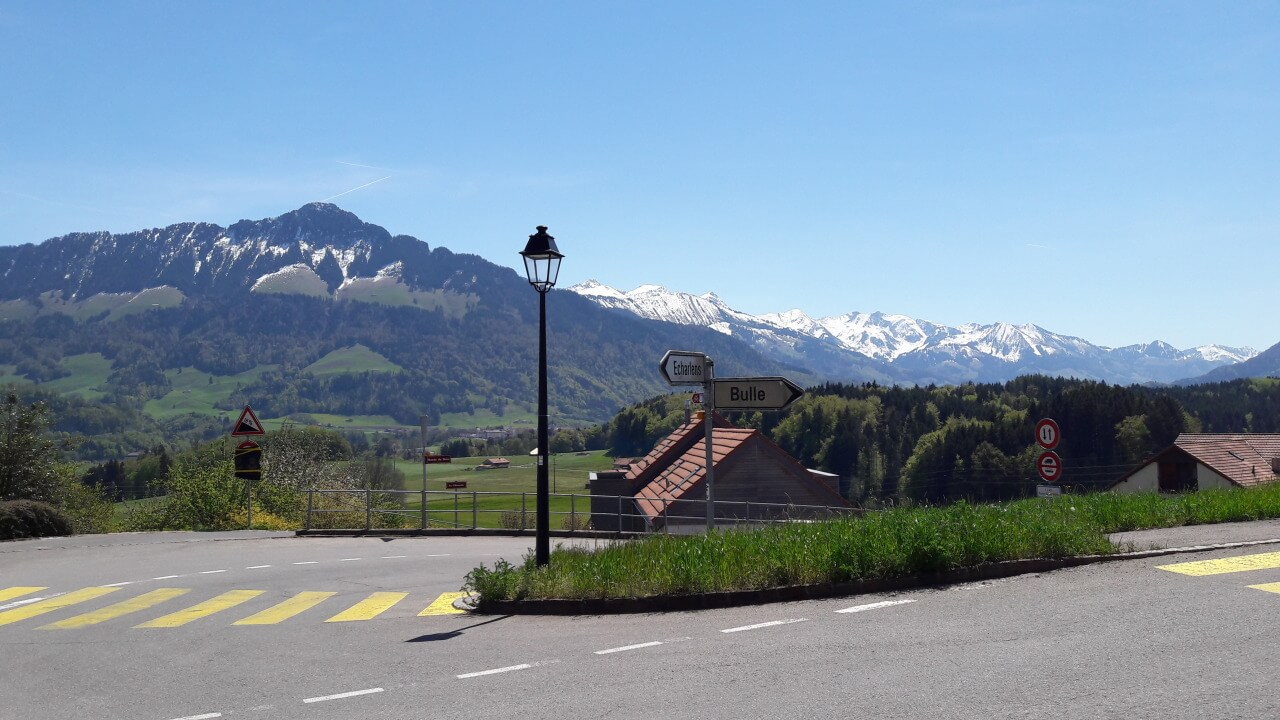
\includegraphics [width=0.3\textwidth]{../Bilder/Gruyere/8.jpg}}\quad
   \subfloat{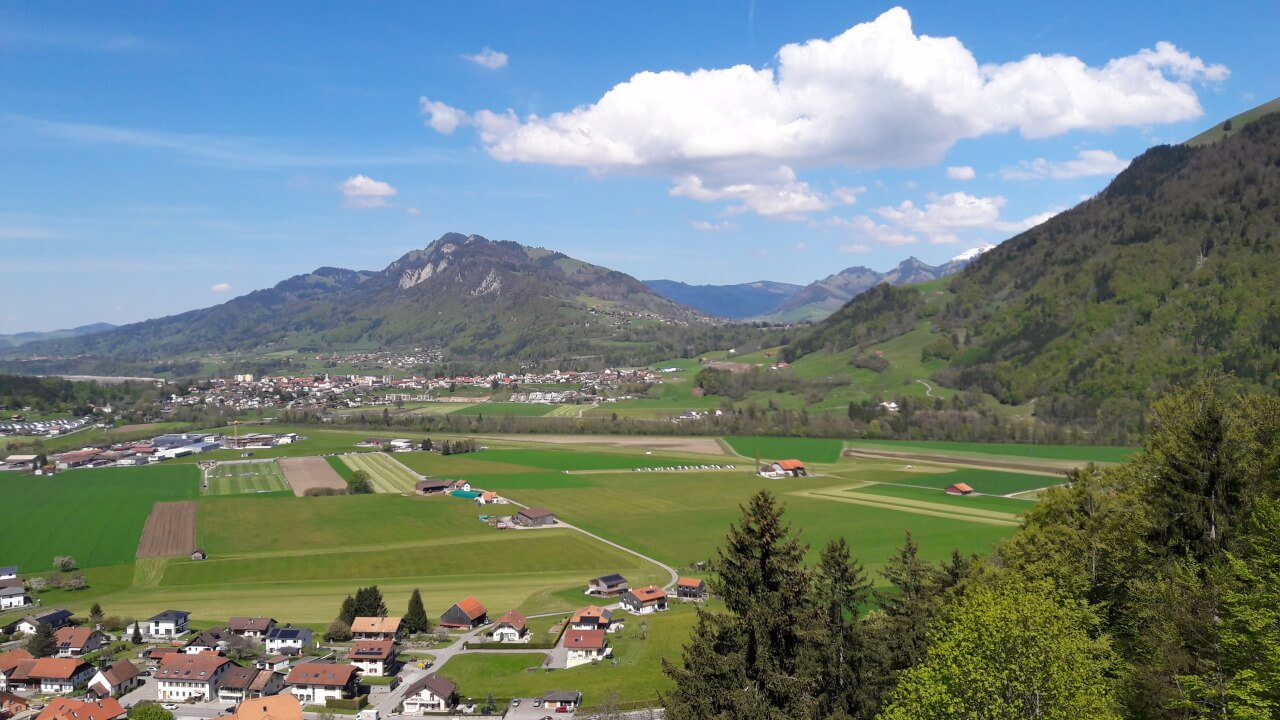
\includegraphics [width=0.3\textwidth]{../Bilder/Gruyere/11.jpg}}\quad
   \subfloat{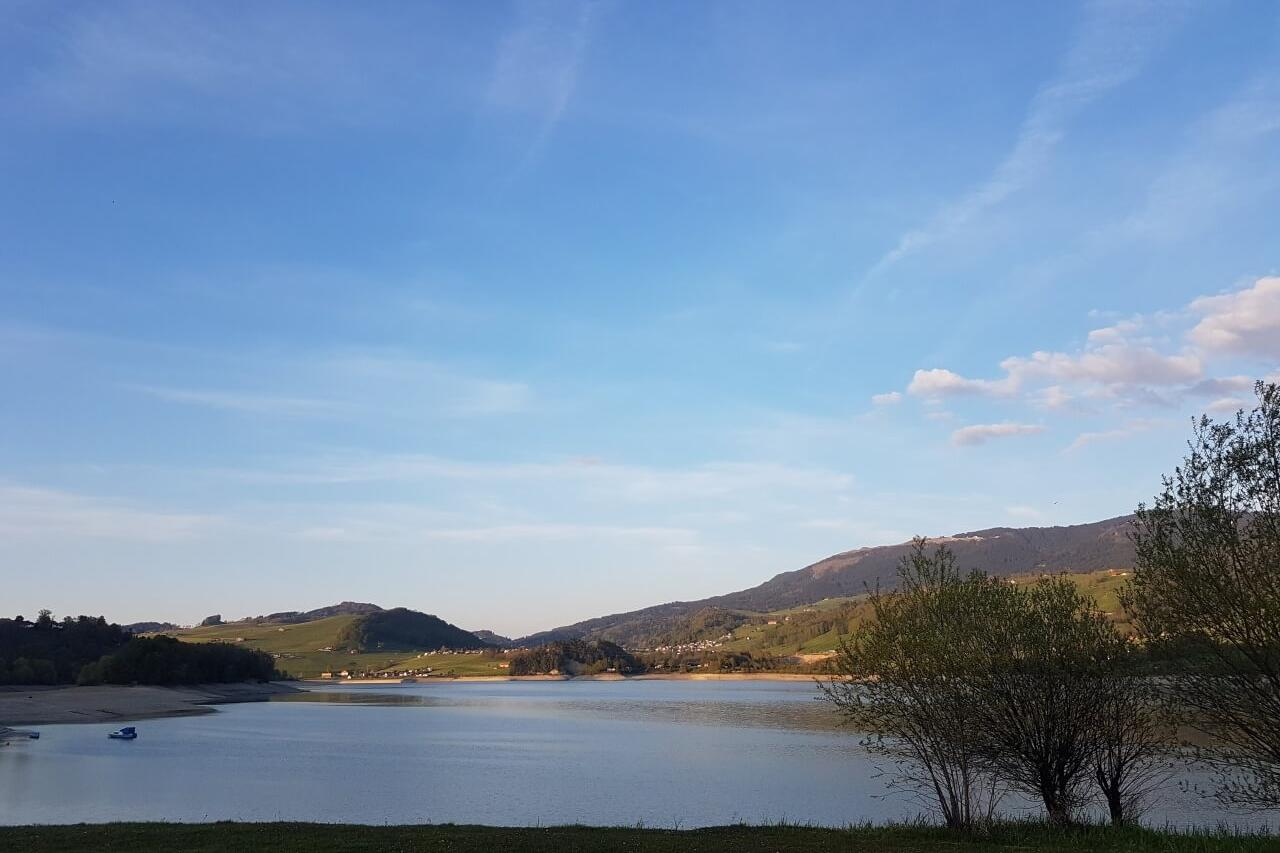
\includegraphics [width=0.3\textwidth]{../Bilder/Gruyere/12.jpg}}\quad
   \caption[Impressionen von der Velotour]{Impressionen von der Velotour}
\end{figure}

Nach einer kurzen St�rkung und Besichtigung des Rummels war es an der Zeit die M�den Beine (von was eigentlich??) wieder auf dem Velo abzustrampeln.
Bulle war das Ziel.
20 Min sp�ter wurde Bulle erkundet und nach etwas Nahrhaftem abgesucht.
Crepes wurden ausgesucht, da die doch eher fr�he Stunde der Auswahl nicht gerade dienlich war.
Das letzte Teilst�ck ging dann �berraschend flott von statten.
Bald k�nnte die Dusche genossen werden.
Naja, sofern man 50 R�ppler dabei hatte.
Sonst hiess eher kalt zu duschen.
Chantal kann da ein Lied von singen.
Nach einem kurzen Kochversuch im Bus (Suppe und Tee) schl�pften wir in die Schlafs�cke und harrten der Dinge die da kommen.
Der Ofen funktionierte die ersten 10 Minuten problemlos.
Dann war jedoch f�r andere auch Schlafenszeit und die Sicherung wurde �berbeansprucht.
Doch irgendeine gute Seele gab ihr eine zweite Chance und hat sie wieder rein gemacht.
Dies verhinderte eine weitere kalte Nacht.

\subsection{07.05.2016 Creux du Van}

\begin{wrapfigure}{L}{0.45\textwidth} 
  \begin{centering}
    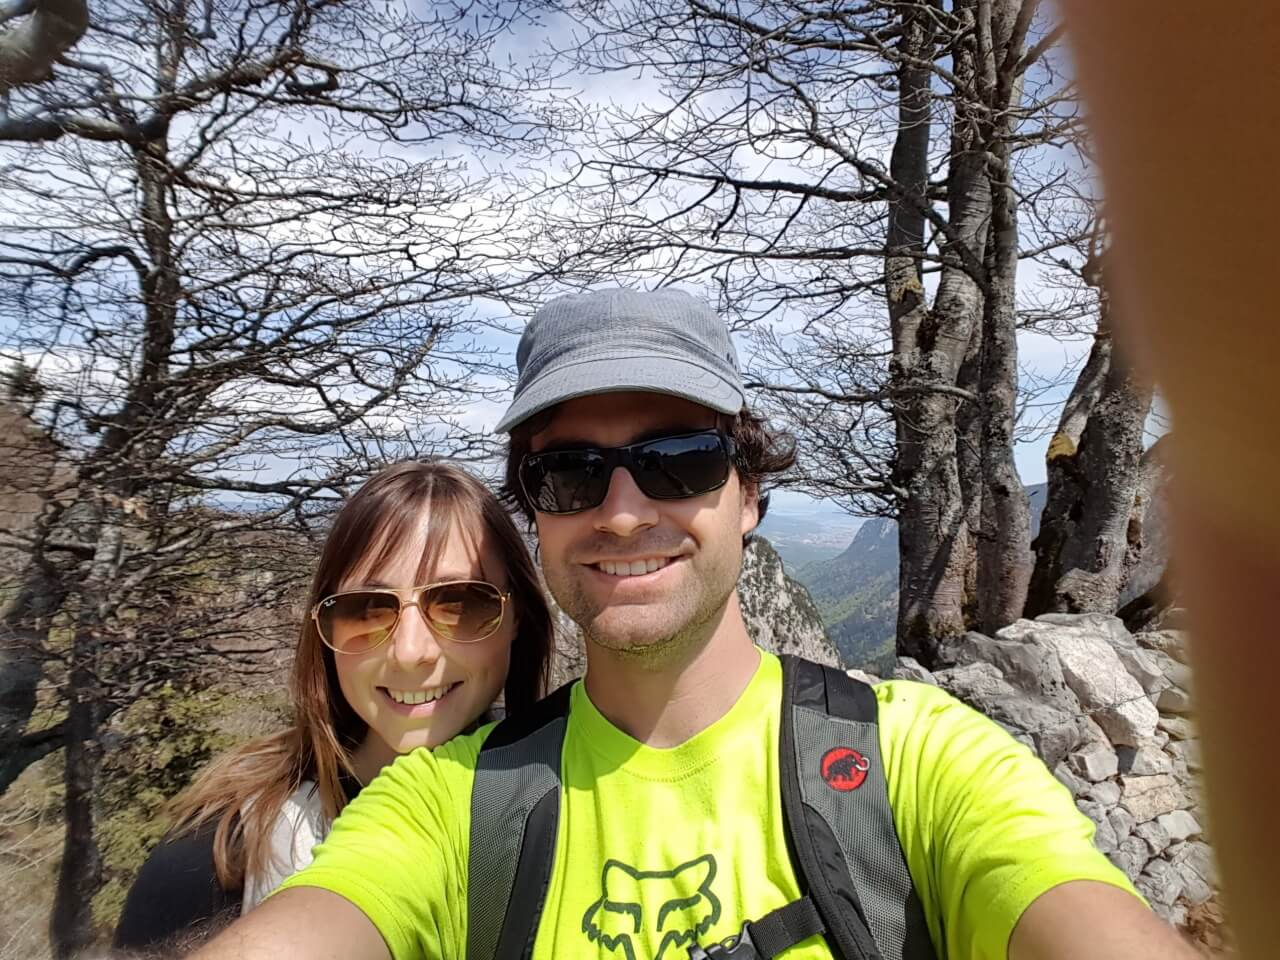
\includegraphics[width=0.4\textwidth, height=5cm, keepaspectratio]{../Bilder/Gruyere/17.jpg}
    \caption{Selfie vor der bekannten Wand}
  \end{centering}
\end{wrapfigure} 

Heute hiess es: Fahrt an den Neuenburger-See und Wanderung auf den Creux du Van.
Nach einer erholsamen Nacht (sch�n warm).
Wurde das n�tigste Zusammengepackt und die anderen Campingbewohner mit einer sch�nen Rauchwolke zu ihrem Morgenessen begr�sst.
Los ging es.
Kreuz und Quer ging es durch das Welschland und das bei sch�nstem Wetter.
Dank Kollege Google fanden wir auch das kleine D�rfchen Noiraigue, der Ausgangspunkt unserer Wanderung.
Kurz vor dem Ankommen mussten noch die Spritvorr�te sowie die Verpflegung aufgefrischt werden.
Saucisse � l'ail fand den Weg in den Einkaufskorb.
Mit etwas Gl�ck konnten wir einen der letzten Parkpl�tze erhaschen.
Ab in die Wanderschuhe und los Richtung Bahnhof.
Den Weg kann man jetzt wirklich nicht verfehlen.
Etliche Personen hatten den gleichen Plan.
Ungef�hr nach der H�lfte des Aufstiegs befindet sich ein Hof, welcher Leckereien verkauft.

Diese Chance musste nat�rlich gepackt werden.
Nach zweieinhalb Stunden Aufstieg erreichten wir die Krete und konnten ein erstes Mal die imposante Wand bestaunen.
Das einzig unsch�ne: 300 Meter vom Abriss entfernt war ein Restaurant, welches mit dem Auto erreichbar ist.
Dementsprechend viele Besucher lockte dieser Ort, welcher noch leicht erreichbar ist an.

Nach einem Picknick und der Erkenntnis, dass die Tagesform einen riesigen Unterschied macht, ging es noch bis zum Punkt le Soliat.
Von dort hiess es die vorher gemachten 700 H�henmeter in Muskelkater umzuwandeln.
Immer runter ging es bis wir nach 1 3/4 Stunden zufrieden und eigentlich noch ganz fit wieder ankamen.
Nur Chantals Beine wollten das ewige Bremsen nicht so recht gefallen und so musste ein Stock als Hilfe beschafft werden.

\begin{figure}[h]
   \centering
      %\subfloat[CAPTION]{BILDERCODE}\qquad
   \subfloat{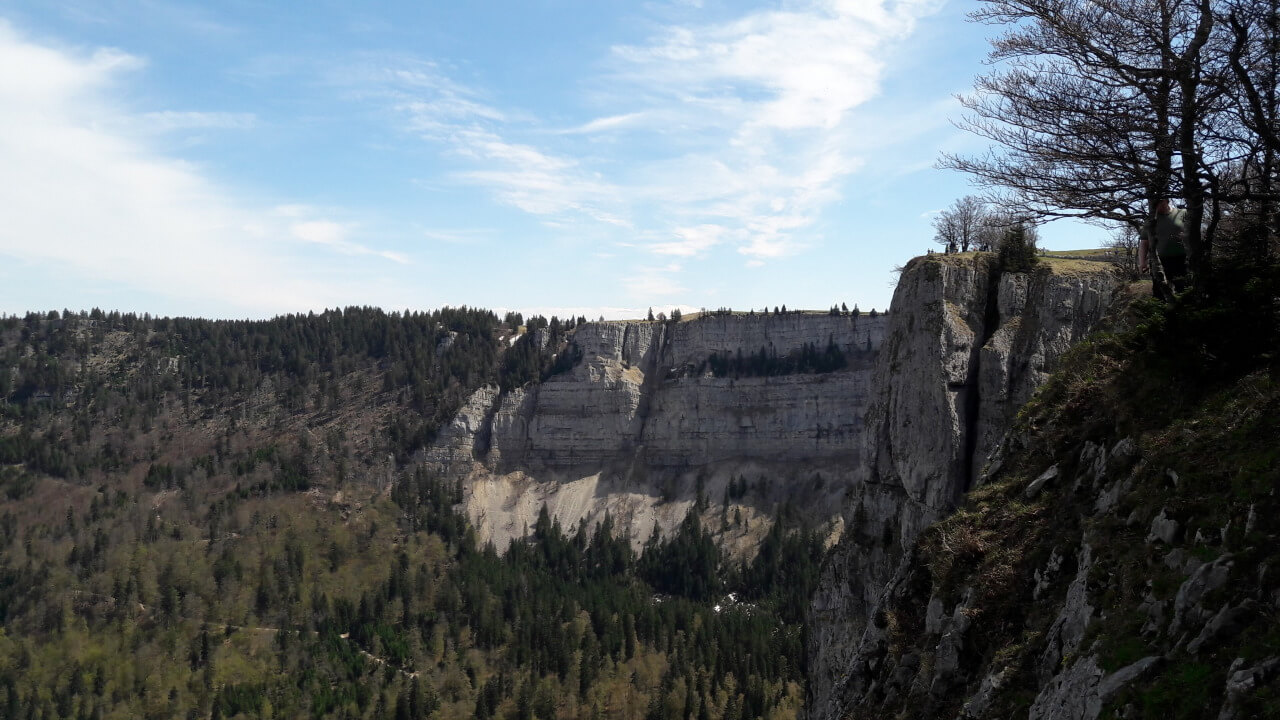
\includegraphics [width=0.3\textwidth]{../Bilder/Gruyere/19.jpg}}\quad
   \subfloat{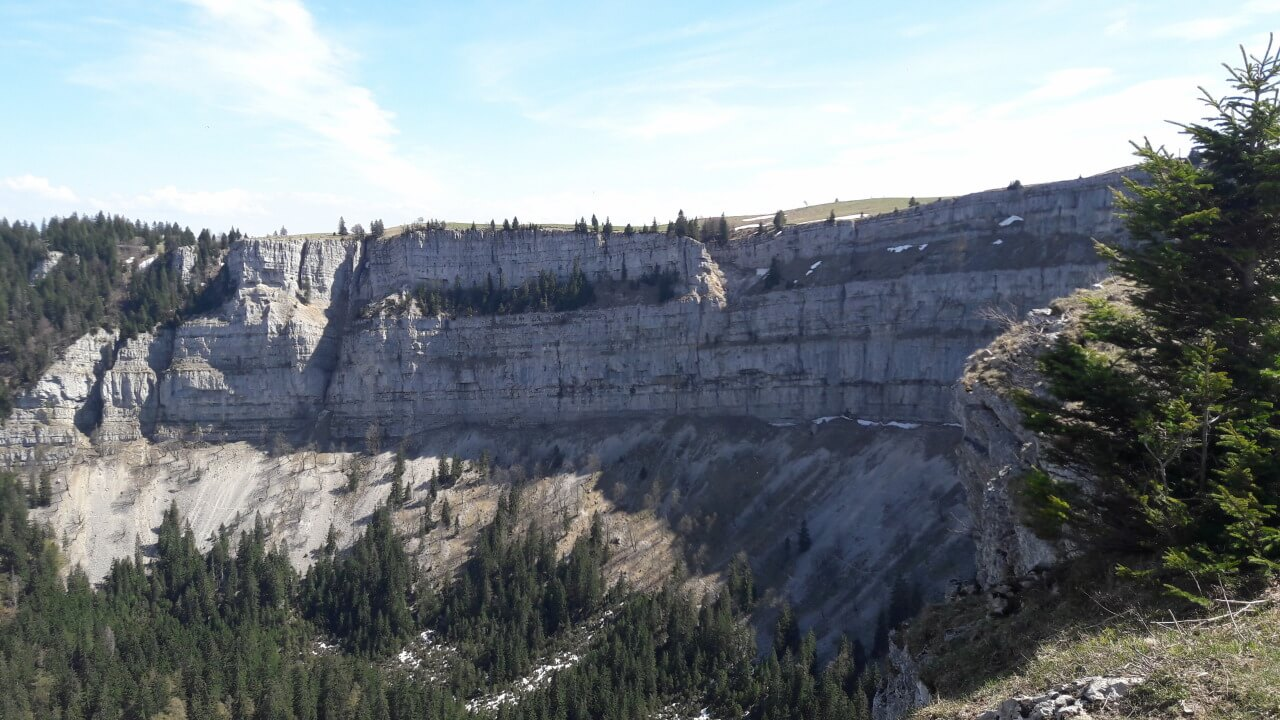
\includegraphics [width=0.3\textwidth]{../Bilder/Gruyere/20.jpg}}\quad
   \subfloat{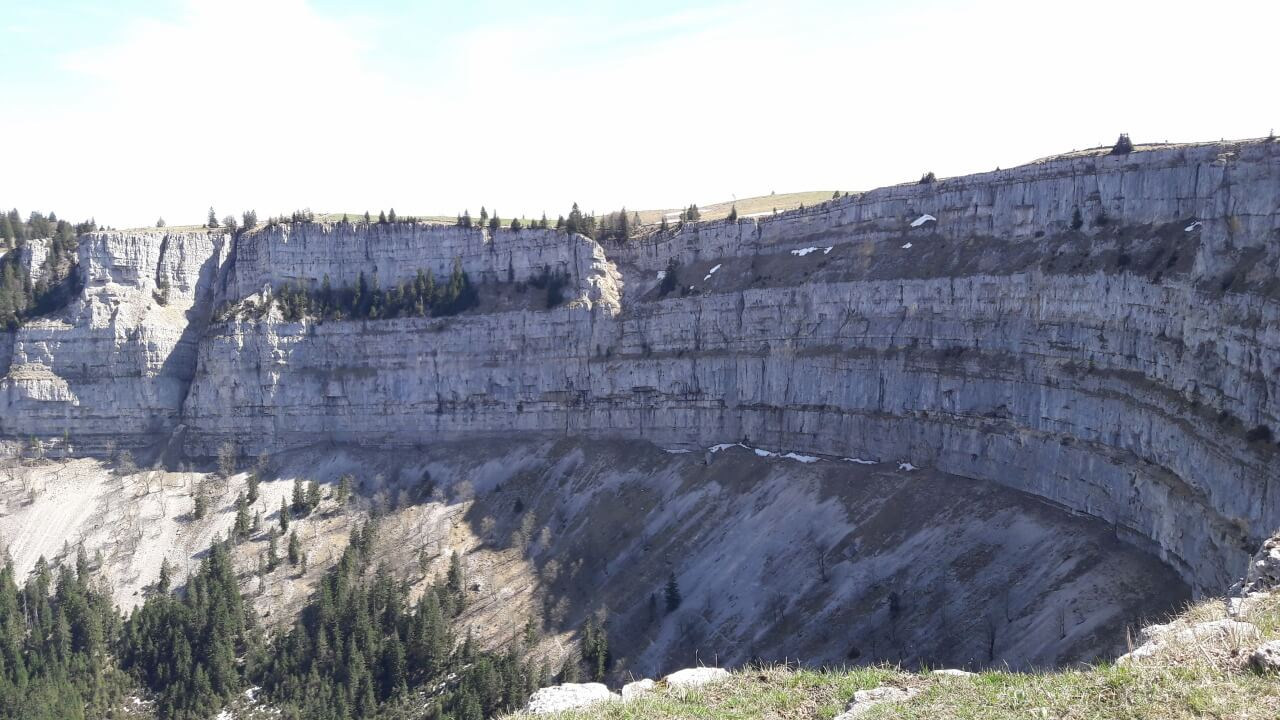
\includegraphics [width=0.3\textwidth]{../Bilder/Gruyere/21.jpg}}\quad
   \caption[Creux du van]{Creux du van}
\end{figure}

Wie schon das ganze Weekend waren auch hier wieder unz�hlige VW Busse unterwegs.
Die Fahrt zur�ck wurde nur durch eine extensive Anordnung von unn�tigen Kreiseln unterbrochen.
Teilweise reichte der Platz zwischen zwei Kreisel nicht einmal f�r ein St�ck Strasse.
So wuchsen zwei Kreisel zusammen.
Da wir eh an dem Camping-Restaurant vorbei mussten, war es nahe liegend gleich noch da zu reservieren.
Nach der Dusche und einem feinen Essen Fischkn�sperli (wie man hier zu sagen pflegt) ginge es f�r eine weitere (leider die letzte Nacht im VW Bus, in dem uns die Heizung gl�cklicherweise nicht im Stich lies.

\begin{figure}[hb]
    \centering
    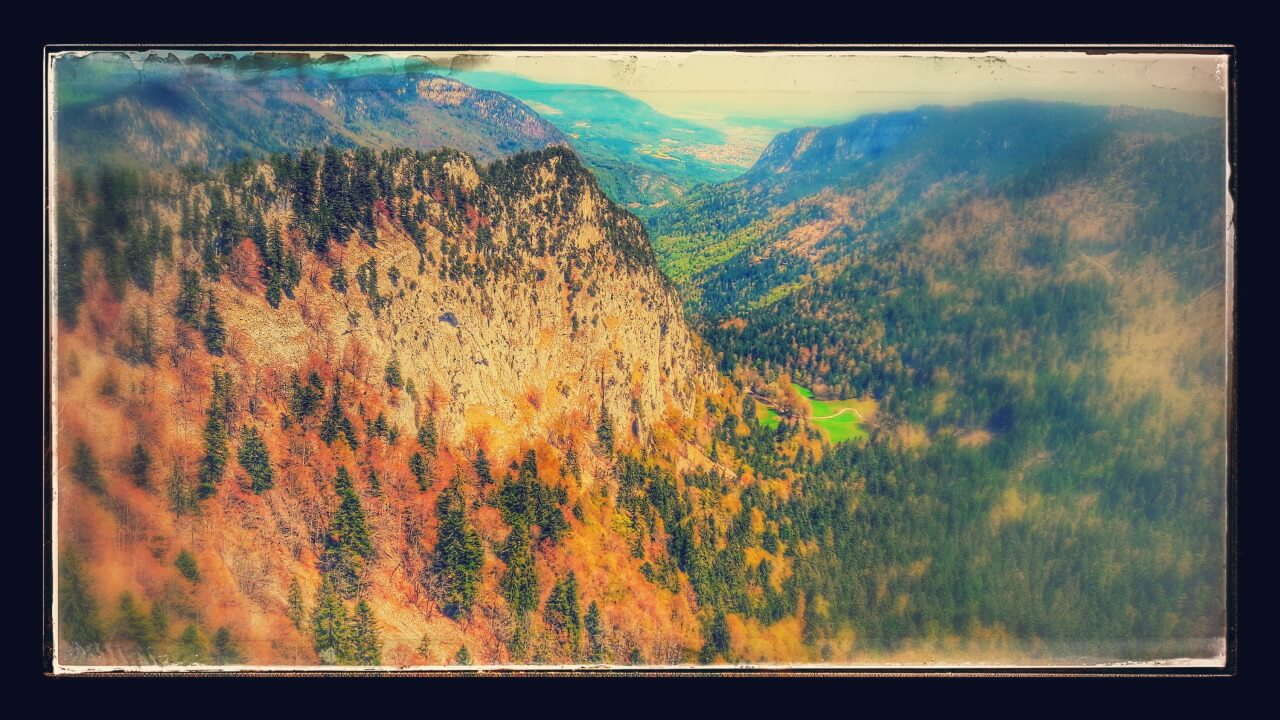
\includegraphics[width=\textwidth]{../Bilder/Gruyere/18.jpg}
    \caption{Creux du van}
    \label{img:Flims}
\end{figure}

\subsection{08.05.2016 Retour und Fribourg}

\begin{wrapfigure}{L}{0.45\textwidth} 
  \begin{centering}
    
\includegraphics[width=0.4\textwidth, height=5cm, keepaspectratio]{../Bilder/Gruyere/26.jpg}
    \caption{PIZZAAAAA}
  \end{centering}
\end{wrapfigure} 

Chantal war schon fr�h auf den Beinen und bevor ich mich �berhaupt das erste Mal bewegte stand das Fr�hst�ck schon bereit.
Es brach richtiggehend Hektik aus und der ganze Campingplatz schien sich auf den Weg zu machen.
�berall wurde Gepackt, verstaut und losgefahren.
Auch wir setzten uns um 11 in den Bus und machten uns auf den Weg Richtung Fribourg.
Ein Parkplatz war schnell gefunden und das angenehme Wetter lud zu einer kleinen Stadtbesichtigung ein.
Die bessere H�lfte fand sich vor einer Unmenge an interessanten Gesch�ften, welche zum Gl�ck eines gemeinsam hatten: Sie waren geschlossen.
Eine Pizzeria zog mich magisch in den Bann und schon bald sassen wir das und genossen ein Mittagessen an der Sonne.

Der R�ckweg �ber die Autobahn war dann ereignislos.
Schon bald konnten wir das ganze Spiel mit Gep�ck, Essen und Velos verladen ein weiteres mal machen und den Bus wieder auf den bekannten und gesch�tzten Parkplatz stellen.
Nach vier kurzen Tagen im Welschland bleibt folgendes zu sagen:

Res�mee (das Wort gibt es tats�chlich so) 

\begin{itemize}
    \item Knoblauchwurst, Brot und Bier in Kombination schl�gt alles Doping der Welt.

    \item Der Mond ist am Lac de Gruyere nicht sichtbar (fragt Chantal f�r Details)

    \item Franz�sisch zu sprechen ist und bleibt m�hsam

    \item Trotzdem lohnt sich der Besuch auf der anderen Seite des R�stigrabens auf jeden Fall

    \item Chantal w�rde auch als Gandalf eine gute Figur machen

    \item Multimediasystem im Bus,  Sch�n und gut aber unn�tz.

    \item Neues Dach daf�r leider geil

    \item Fribourg auf jeden Fall wieder einmal ein Besuch wert!
\end{itemize}

\newpage

\begin{figure}[H]
    \centering
    
\includegraphics[width=\textwidth,height=14cm, keepaspectratio]{../Bilder/Logo/Logo_trans.png}
    \label{img:Logo}
\end{figure}
\vfill
    \begin{center}
        {\huge  Weitere Informationen zum Bus und unseren Reisen sind auf der Homepage {\url{www.jackthebus.com}} zu finden}
\end{center}

\end{document}
